% Task 3: one keystream, two messages. Values from Task3/reuse.py;
% CHECKED (python3): C1 XOR P1 starts with 0xA6 XOR 0x4D ('M') = 0xEB;
%   0xBF XOR 0xEB = 0x54 = 'T'. The other bytes are the result of the task: not shown.
\documentclass[12pt,tikz,border=6pt]{standalone}
% Shared preamble of the task figures of Lecture 1.
% The colours and styles are copied from the preamble of ../main.tex (keep them in sync).
\usepackage{lmodern}
\usepackage[T1]{fontenc}
\renewcommand{\familydefault}{\sfdefault}
\usepackage{amsmath,amssymb}
\usepackage{xcolor}
\usepackage{fontawesome5}
\usetikzlibrary{arrows.meta, calc, positioning, fit, decorations.pathreplacing, decorations.pathmorphing, backgrounds}

% ---------- template ----------
\definecolor{DeepBlue}{HTML}{283593}
\definecolor{AccentOrange}{HTML}{EB5A14}
\definecolor{LightGray}{HTML}{F5F6FA}
% ---------- actors and categories (S1 to S6) ----------
\definecolor{sIndigo}{HTML}{5C6BC0}   % the sender
\definecolor{sPink}{HTML}{EC407A}     % the attacker
\definecolor{sViolet}{HTML}{7E57C2}   % plaintext
\definecolor{sAmber}{HTML}{FFB300}    % key and keystream
\definecolor{sTeal}{HTML}{26A69A}     % the receiver
\definecolor{sBrown}{HTML}{8D6E63}    % ciphertext
\definecolor{sPinkText}{HTML}{C2185B}
\definecolor{sAmberText}{HTML}{A06A00}
\definecolor{sTealText}{HTML}{00796B}
% ---------- actions and results ----------
\definecolor{aExec}{HTML}{43A047}
\definecolor{aRead}{HTML}{1E88E5}
\definecolor{aWrite}{HTML}{E53935}
% ---------- neutral ----------
\definecolor{nInk}{HTML}{37474F}
\definecolor{nLine}{HTML}{90A4AE}
\definecolor{nLight}{HTML}{CFD8DC}
\definecolor{nFill}{HTML}{ECEFF1}
\definecolor{nIdle}{HTML}{E0E0E0}

% ---------- TikZ styles (as in main.tex; byte cells a little larger for the web) ----------
\tikzset{
  hw/.style={draw=nLine, thick, fill=nFill, text=nInk, rounded corners=3pt, align=center, inner sep=4pt},
  hwmain/.style={draw=nInk, thick, fill=nInk, text=white, rounded corners=3pt, align=center, inner sep=4pt},
  cell/.style={draw=nLine, thick, fill=white, text=nInk, font=\ttfamily\small},
  cellfree/.style={cell, dashed, draw=nLight},
  container/.style={draw=nLine, thick, dashed, rounded corners=5pt},
  actor/.style={fill=#1, draw=#1, text=white, rounded corners=3pt, align=center, font=\small\bfseries, inner sep=5pt},
  actorlight/.style={fill=#1!15, draw=#1, thick, text=nInk, rounded corners=3pt, align=center, inner sep=5pt},
  data/.style={-{Stealth}, very thick, nInk},
  flow/.style={-{Stealth}, very thick, DeepBlue},
  annot/.style={draw=AccentOrange, line width=1.6pt, rounded corners=3pt},
  byte/.style={draw=nLine, thick, fill=white, text=nInk, font=\ttfamily\small,
    minimum width=0.8cm, minimum height=0.62cm, inner sep=1pt, rounded corners=1.5pt},
  ptb/.style={byte, fill=sViolet!15, draw=sViolet},
  ksb/.style={byte, fill=sAmber!25, draw=sAmber},
  ctb/.style={byte, fill=sBrown!15, draw=sBrown},
  unk/.style={byte, fill=white, dashed, text=sViolet},
  rowlabel/.style={font=\small\bfseries, text=nInk, anchor=east},
  note/.style={font=\small, text=nInk},
  bigxor/.style={circle, draw=nInk, very thick, fill=white, inner sep=0pt, minimum size=0.8cm, font=\Large},
  radio/.style={-{Stealth}, very thick, nInk, decorate,
    decoration={snake, amplitude=1.2pt, segment length=7pt, post length=4pt}},
  % a white card behind the whole figure, so that it stays readable in a dark theme
  card/.style={show background rectangle, background rectangle/.style={fill=white, draw=none}, inner frame sep=8pt},
}
% a row of bytes: \byterow{x of the first cell}{y}{style}{list of values}{step between cells}
\newcommand{\byterow}[5]{%
  \expandafter\def\expandafter\brlist\expandafter{#4}%
  \foreach \v [count=\k from 0] in \brlist {
    \node[#3] at ({#1+#5*\k},#2) {\v};
  }}
% the generator / cipher box: dark, with cogs. \cogbox{name}{position}{label}{width}
\newcommand{\cogbox}[4]{%
  \node[hwmain, minimum width=#4, minimum height=1.3cm] (#1) at (#2) {};
  \node[text=white, font=\Large] at ([yshift=0.22cm]#1.center) {\faCogs};
  \node[text=white, font=\small\bfseries] at ([yshift=-0.32cm]#1.center) {#3};}
\newcommand{\ok}{\textcolor{aExec}{\faCheck}}
\newcommand{\nok}{\textcolor{aWrite}{\faTimes}}
\newcommand{\badge}[1]{\tikz[baseline=(b.base)]\node[circle,fill=AccentOrange,text=white,
  inner sep=1.5pt,font=\bfseries\footnotesize] (b) {#1};}

\begin{document}
\pagecolor{white}
\begin{tikzpicture}[>=Stealth]
  \def\dx{0.92}
  % the story: one keystream Z for two messages, the attacker has C1, C2 and P1
  \node[circle, fill=sPink, text=white, minimum size=1.0cm, font=\Large] (a) at (-1.4,2.0) {\faUserSecret};
  \node[note, anchor=west, align=left] at (-0.7,2.0)
    {You recorded \textbf{C1} and \textbf{C2}. Both were encrypted with \textbf{the same keystream Z}:\\
     \texttt{C1 = P1 XOR Z}\quad and\quad \texttt{C2 = P2 XOR Z}.\quad You also know \textbf{P1}.};

  \foreach \k in {0,...,14} \node[font=\small, text=gray] at ({\dx*\k},0.9) {\k};
  % step 2: the keystream from C1 and P1
  \node[font=\normalsize\bfseries, text=nInk, anchor=west] at (-3.3,0.3) {\badge{2}\ Get Z};
  \node[rowlabel] at (-0.5,-0.3) {C1};
  \byterow{0}{-0.3}{ctb}{A6,DA,32,D5,97,79,8F,52,E6,4D,6A,11,47,E6,0F}{\dx}
  \node[rowlabel] at (-0.5,-1.05) {XOR\ \ P1};
  \byterow{0}{-1.05}{ptb, font=\ttfamily\normalsize\bfseries}{M,E,E,T,{\textvisiblespace},M,E,{\textvisiblespace},A,T,{\textvisiblespace},9,{\textvisiblespace},P,M}{\dx}
  \draw[nInk, thick] (-0.45,-1.48) -- ({14.45*\dx},-1.48);
  \node[rowlabel] at (-0.5,-1.9) {= Z};
  \node[ksb] at (0,-1.9) {EB};
  \foreach \k in {1,...,14} \node[byte, fill=white, dashed, draw=sAmber, text=sAmberText] at ({\dx*\k},-1.9) {?};

  % step 3: Z opens the second message
  \node[font=\normalsize\bfseries, text=nInk, anchor=west] at (-3.3,-2.75) {\badge{3}\ Open C2};
  \node[rowlabel] at (-0.5,-3.35) {C2};
  \byterow{0}{-3.35}{ctb}{BF,D7,32,A1,E7,7D,84,52,EE,4A,6A,1C,56,81,70}{\dx}
  \node[rowlabel] at (-0.5,-4.1) {XOR\ \ Z};
  \node[ksb] at (0,-4.1) {EB};
  \foreach \k in {1,...,14} \node[byte, fill=white, dashed, draw=sAmber, text=sAmberText] at ({\dx*\k},-4.1) {?};
  \draw[nInk, thick] (-0.45,-4.53) -- ({14.45*\dx},-4.53);
  \node[rowlabel] at (-0.5,-4.95) {= P2};
  \node[ptb, font=\ttfamily\normalsize\bfseries] at (0,-4.95) {T};
  \foreach \k in {1,...,14} \node[unk] at ({\dx*\k},-4.95) {?};

  % the first column, worked out
  \draw[annot] (-0.46,-5.35) rectangle (0.46,0.05);
  \node[font=\small, text=AccentOrange, anchor=north west, align=left] at (-0.46,-5.5)
    {\texttt{0xA6 XOR \textquotesingle M\textquotesingle\ = 0xEB}, then \texttt{0xBF XOR 0xEB = 0x54 = \textquotesingle T\textquotesingle}.
     \ \ No key needed: \texttt{C1 XOR P1 = Z}.};
\end{tikzpicture}
\end{document}
